\documentclass[pdf]{beamer}
\usepackage{graphicx}
\mode<presentation>{}
\title{LibEuFin}
\subtitle{Libre European Finance}
\author{Marcello Stanisci}
\newcommand{\boldred}[1]{\textcolor{red}{\textbf{#1}}}
\begin{document}

\begin{frame}
  \titlepage
\end{frame}

\begin{frame}
  \begin{center}
  \boldred{People} and businesses need \boldred{programmatic access} to bank accounts, and
  the \boldred{EU} recognized this by passing the 2nd Payment Service Directive.

  But it's extremely \boldred{complicated}!
  \end{center}
\end{frame}

\begin{frame}{Too many protocols..}
  \begin{itemize}
    \item EBICS: hundreds of pages, just for {\it enclosing} payloads
    \item ISO20022: hundreds of pages for payloads
    \item FinTS / HBCI: hundreds of pages
    \item NextGenPSD2 by Berlin Group 
    \item Startup banks: N26 / Revoult
    \item 100\% proprietary: PayPal
    \item ..
  \end{itemize}
\end{frame}

\begin{frame}{LibEuFin}
  \begin{center}
  LibEuFin is an Open Source \boldred{service} and \boldred{API} that allows
  developers communities and SMEs to programmatically \boldred{access their bank accounts}.

  It \boldred{abstracts} over complex \boldred{legacy APIs} and provides a bank \boldred{sandbox}
  to make testing cheap and easy.
  \end{center}
\end{frame}

\begin{frame}{Improvements}
  \begin{itemize}
  \item \boldred{Unifies} several banking protocols into an abstraction layer.
  \item Enables development of FinTech apps \boldred{without "clouds" or third parties}
  \item \boldred{Frees} application developers from implementing \boldred{difficult cryptography}
  \end{itemize}
\end{frame}

\begin{frame}{Architecture}
  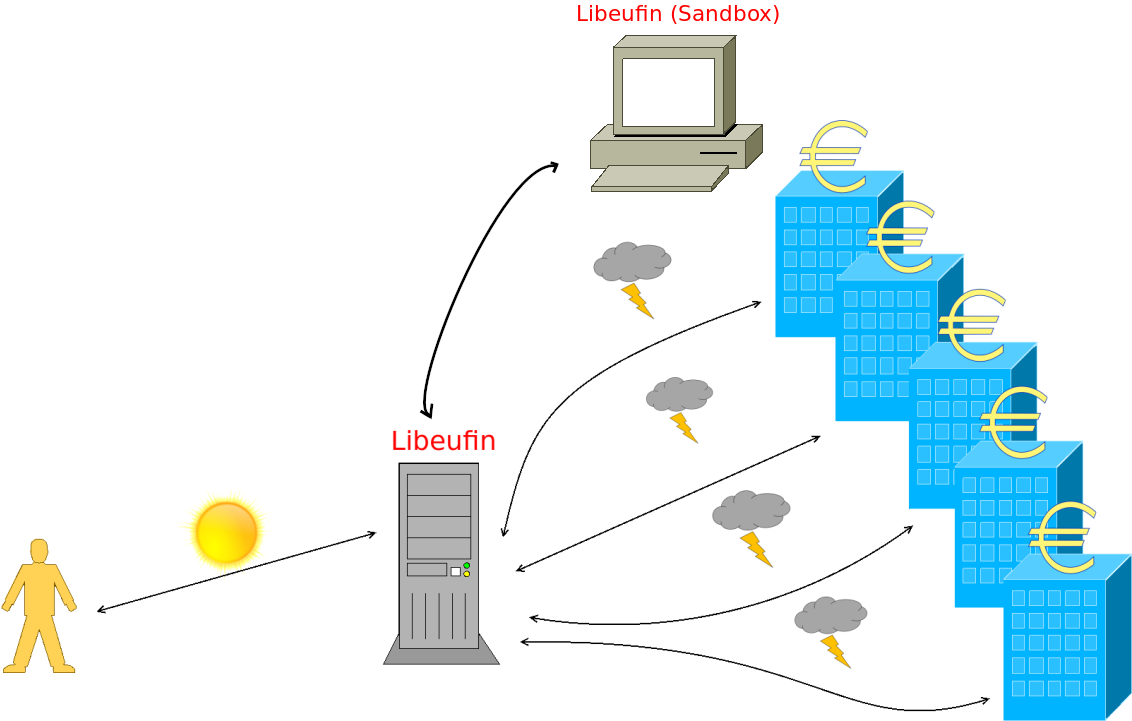
\includegraphics[height=0.63\textheight]{libeufin.png}
\end{frame}

\begin{frame}{Current status}
  \begin{itemize}
    \item One major protocol (\boldred{EBICS}) implemented
    \item Current code works with \boldred{real bank account} at GLS!
    \item Should work with all banks of the \boldred{German Credit Union}
    \item Ongoing \boldred{integration with Taler} (former PF project).
  \end{itemize}
\end{frame}

\begin{frame}{Challenges}
  \begin{itemize}
    \item \boldred{Slow communication} with banks.
    \item \boldred{Significant research} needed before starting coding.
    \item \boldred{Subscriber initiation} process: mixes digital and analog!
    \item No reliable \boldred{testing environment} available.
  \end{itemize}
\end{frame}

\begin{frame}{Successes}
  \begin{itemize}
    \item \boldred{Milestones estimation} was (almost!) accurate.
    \item Our approach to testing (develop \boldred{sandbox first}) was successful: Real bank access
          worked on first try, after 4 months of development.
  \end{itemize}
\end{frame}

\begin{frame}{Future}
  \begin{center}
  LibEuFin will be \boldred{further developed} for the \boldred{next 2 years},
  thanks to our employment at \boldred{Taler Systems}.
  \end{center}
\end{frame}

\begin{frame}{Where to find us}
  \begin{center}
  Web: \\ \textcolor{red}{\tt{https://libeufin.tech}} \\
  e-mail: \\ \textcolor{red}{\tt{contact@libeufin.tech}}
  \end{center}
\end{frame}

\end{document}
